\documentclass[11pt]{article}\usepackage[]{graphicx}\usepackage[]{color}
%% maxwidth is the original width if it is less than linewidth
%% otherwise use linewidth (to make sure the graphics do not exceed the margin)
\makeatletter
\def\maxwidth{ %
  \ifdim\Gin@nat@width>\linewidth
    \linewidth
  \else
    \Gin@nat@width
  \fi
}
\makeatother

\definecolor{fgcolor}{rgb}{0.345, 0.345, 0.345}
\newcommand{\hlnum}[1]{\textcolor[rgb]{0.686,0.059,0.569}{#1}}%
\newcommand{\hlstr}[1]{\textcolor[rgb]{0.192,0.494,0.8}{#1}}%
\newcommand{\hlcom}[1]{\textcolor[rgb]{0.678,0.584,0.686}{\textit{#1}}}%
\newcommand{\hlopt}[1]{\textcolor[rgb]{0,0,0}{#1}}%
\newcommand{\hlstd}[1]{\textcolor[rgb]{0.345,0.345,0.345}{#1}}%
\newcommand{\hlkwa}[1]{\textcolor[rgb]{0.161,0.373,0.58}{\textbf{#1}}}%
\newcommand{\hlkwb}[1]{\textcolor[rgb]{0.69,0.353,0.396}{#1}}%
\newcommand{\hlkwc}[1]{\textcolor[rgb]{0.333,0.667,0.333}{#1}}%
\newcommand{\hlkwd}[1]{\textcolor[rgb]{0.737,0.353,0.396}{\textbf{#1}}}%

\usepackage{framed}
\makeatletter
\newenvironment{kframe}{%
 \def\at@end@of@kframe{}%
 \ifinner\ifhmode%
  \def\at@end@of@kframe{\end{minipage}}%
  \begin{minipage}{\columnwidth}%
 \fi\fi%
 \def\FrameCommand##1{\hskip\@totalleftmargin \hskip-\fboxsep
 \colorbox{shadecolor}{##1}\hskip-\fboxsep
     % There is no \\@totalrightmargin, so:
     \hskip-\linewidth \hskip-\@totalleftmargin \hskip\columnwidth}%
 \MakeFramed {\advance\hsize-\width
   \@totalleftmargin\z@ \linewidth\hsize
   \@setminipage}}%
 {\par\unskip\endMakeFramed%
 \at@end@of@kframe}
\makeatother

\definecolor{shadecolor}{rgb}{.97, .97, .97}
\definecolor{messagecolor}{rgb}{0, 0, 0}
\definecolor{warningcolor}{rgb}{1, 0, 1}
\definecolor{errorcolor}{rgb}{1, 0, 0}
\newenvironment{knitrout}{}{} % an empty environment to be redefined in TeX

\usepackage{alltt}

\usepackage[margin=1in,bottom=.5in,includehead,includefoot]{geometry}
\usepackage{hyperref}
\usepackage{alltt}
\usepackage{fancyhdr}
\pagestyle{fancy}
\fancyhf{}

\title{Open Intro Biostat R Companion: \\ Chapter 1}
\author{Morgan F. Breitmeyer}
\date{}
\IfFileExists{upquote.sty}{\usepackage{upquote}}{}
\begin{document}

\maketitle

\tableofcontents

\vspace{1cm}
This document is intended to be a companion source to the textbook \textit{Introductory Statistics for the Life and Biomedical Sciences} that goes through all of the $R$ code and operations seen in the text.

We have created a package that stores all of the datasets seen in the text.  You can download the package using the following command:
%% These commands aren't going to work until we have uploaded the package to CRAN. Just skip it for now and require below.
\begin{knitrout}
\definecolor{shadecolor}{rgb}{0.969, 0.969, 0.969}\color{fgcolor}\begin{kframe}
\begin{alltt}
\hlkwd{install.packages}\hlstd{(}\hlstr{"OIBioStat"}\hlstd{)}  \hlcom{## make sure to include the quotations}
\end{alltt}
\end{kframe}
\end{knitrout}

The above command only needs to be run once, as after that, the package will be in your computer.  However, each time you want to use the package, you must alert $R$ using the following command:
\begin{knitrout}
\definecolor{shadecolor}{rgb}{0.969, 0.969, 0.969}\color{fgcolor}\begin{kframe}
\begin{alltt}
\hlkwd{require}\hlstd{(OIBioStat)} \hlcom{## note the lack of quotations here}
\end{alltt}
\end{kframe}
\end{knitrout}

\section{Case study: preventing peanut allergies}
%% Perhaps make a preface. Also consider a chapter 0 with basics of R and maybe how to download it?

The first dataset encountered in the text is from the ``Learning Early About Peanut Allergy" (LEAP) study.  The dataset contains the results of a study conducted in 2015, which was reported in the \textit{New England Journal of Medicine.}  There are several basic things we can do to learn about our dataset.  Firstly, we can see the help files that come with it, using the following command:

\begin{knitrout}
\definecolor{shadecolor}{rgb}{0.969, 0.969, 0.969}\color{fgcolor}\begin{kframe}
\begin{alltt}
\hlkwd{help}\hlstd{(LEAP)}
\end{alltt}
\end{kframe}
\end{knitrout}
Running this, you should see a file appear, which contains several useful pieces of information:
\begin{itemize}
\item \textbf{Description:} This is a very short description of the dataset.  It typically contains a short overview of what is contained, but few details.
\item \textbf{Format:} This is typically the most useful section of the help file.  It contains the names and descriptions of every variable in the dataset.  It should contain information such as the units and the type of variable seen.  A variable can take two main types: a \textit{factor} meaning it can be one of several set categories which do not have quantitative meaning (such as male and female or racial identification) or a \textit{number} meaning the variable can take on a range of quantitative values, which typically have some sort of meaning (such as height, weight, or frequency).
\item \textbf{Details:} This section is an extension of the Description section seen at the beginning of the help file.  It will typically offer more details about where the data came from and its previous or intended uses.
\end{itemize}
The next important thing to know about datasets is how to take a look at the dataset itself.  The simplest way to do this is as follows:
\begin{knitrout}
\definecolor{shadecolor}{rgb}{0.969, 0.969, 0.969}\color{fgcolor}\begin{kframe}
\begin{alltt}
\hlkwd{View}\hlstd{(LEAP)}
\end{alltt}
\end{kframe}
\end{knitrout}
This command should cause a new window to pop up that shows you the whole dataset.  Here you can see the variable names you saw in your help file across the top as the names of the columns.  Also, you can see the entries in the dataset, as the various values within the rows and columns.  Note that the farthest left column should show what are called indeces, these are computer generated values that allow you to access specific rows in the dataset, but are not meaningful values in the dataset.  It is important to note that these indeces typically have no meaning that corresponds with the data, but are very useful for working with the data.

Another simple way to view a small portion of the data is as follows:
\begin{knitrout}
\definecolor{shadecolor}{rgb}{0.969, 0.969, 0.969}\color{fgcolor}\begin{kframe}
\begin{alltt}
\hlstd{LEAP[}\hlnum{1}\hlopt{:}\hlnum{5}\hlstd{,}\hlnum{1}\hlopt{:}\hlnum{6}\hlstd{]}
\end{alltt}
\begin{verbatim}
##   participant.ID    treatment.group age.months    sex primary.ethnicity
## 1    LEAP_100522 Peanut Consumption     6.0780 Female             Black
## 2    LEAP_103358 Peanut Consumption     7.5893 Female             White
## 3    LEAP_105069   Peanut Avoidance     5.9795   Male             White
## 4    LEAP_105328 Peanut Consumption     7.0308 Female             White
## 5    LEAP_106377   Peanut Avoidance     6.4066   Male             White
##   overall.V60.outcome
## 1            PASS OFC
## 2            PASS OFC
## 3            PASS OFC
## 4            PASS OFC
## 5            PASS OFC
\end{verbatim}
\end{kframe}
\end{knitrout}
This command will print out in the console the first 5 rows of the data.  The bracket notation above after the dataset name implies location, so you are telling $R$ at what location you would like to look.  The notation here is \textit{dataset[rows,columns]}, so the 1:5 dictates the first 5 rows and the 1:6 dictates the first 6 columns.  You can use this notation to access any combination of rows and columns in the dataset that you wish.  If you wanted to tell $R$ to take all the columns, but only the first five rows you could do that with the following:

\begin{knitrout}
\definecolor{shadecolor}{rgb}{0.969, 0.969, 0.969}\color{fgcolor}\begin{kframe}
\begin{alltt}
\hlcom{## note the space (or lack of text after the comma)}
\hlstd{LEAP[}\hlnum{1}\hlopt{:}\hlnum{5}\hlstd{, ]}
\end{alltt}
\begin{verbatim}
##   participant.ID    treatment.group age.months    sex primary.ethnicity
## 1    LEAP_100522 Peanut Consumption     6.0780 Female             Black
## 2    LEAP_103358 Peanut Consumption     7.5893 Female             White
## 3    LEAP_105069   Peanut Avoidance     5.9795   Male             White
## 4    LEAP_105328 Peanut Consumption     7.0308 Female             White
## 5    LEAP_106377   Peanut Avoidance     6.4066   Male             White
##   overall.V60.outcome
## 1            PASS OFC
## 2            PASS OFC
## 3            PASS OFC
## 4            PASS OFC
## 5            PASS OFC
\end{verbatim}
\end{kframe}
\end{knitrout}
This output actually gives the same as the above command, but with a different command.  This is a common theme in $R$ - there are multiple ways to do everything.

The final and most complex way to look at part of the data can be seen below and in Table 1.1 in the text. In this case, rather than doing a list of numbers sequentially, we create a list using the command $c()$ which binds the values inside the parentheses together into a list.  We can see the command below has first a list of row indexes (numbers as described above) and then a list of column names.

\begin{knitrout}
\definecolor{shadecolor}{rgb}{0.969, 0.969, 0.969}\color{fgcolor}\begin{kframe}
\begin{alltt}
\hlcom{## Table 1.1}
\hlstd{LEAP[}\hlkwd{c}\hlstd{(}\hlnum{1}\hlstd{,}\hlnum{2}\hlstd{,}\hlnum{3}\hlstd{,}\hlnum{529}\hlstd{,} \hlnum{530}\hlstd{),}\hlkwd{c}\hlstd{(}\hlstr{"participant.ID"}\hlstd{,} \hlstr{"treatment.group"}\hlstd{,}
                         \hlstr{"overall.V60.outcome"}\hlstd{)]}
\end{alltt}
\begin{verbatim}
##     participant.ID    treatment.group overall.V60.outcome
## 1      LEAP_100522 Peanut Consumption            PASS OFC
## 2      LEAP_103358 Peanut Consumption            PASS OFC
## 3      LEAP_105069   Peanut Avoidance            PASS OFC
## 639    LEAP_994047   Peanut Avoidance            PASS OFC
## 640    LEAP_997608 Peanut Consumption            PASS OFC
\end{verbatim}
\end{kframe}
\end{knitrout}

Another good way to visualize data is using a table, which summarizes the data using two variables, one on each axis, and then provides the number of counts matching the varaible categories.  We can see this with the below command, which corresponds to Table 1.2 in the text.  Using the \textit{table} command, the first variable put in goes to the x-axis (meaning the row names) and the second variable goes to the y-axis (meaning the column names).  The addition of the \textit{addmargins()} command prints the sums of the rows and columns on the sides of the table as seen below,
\begin{knitrout}
\definecolor{shadecolor}{rgb}{0.969, 0.969, 0.969}\color{fgcolor}\begin{kframe}
\begin{alltt}
\hlcom{## Table 1.2}
\hlkwd{table}\hlstd{(LEAP}\hlopt{$}\hlstd{treatment.group, LEAP}\hlopt{$}\hlstd{overall.V60.outcome)}
\end{alltt}
\begin{verbatim}
##                     
##                      FAIL OFC PASS OFC
##   Peanut Avoidance         36      227
##   Peanut Consumption        5      262
\end{verbatim}
\begin{alltt}
\hlkwd{addmargins}\hlstd{(}\hlkwd{table}\hlstd{(LEAP}\hlopt{$}\hlstd{treatment.group, LEAP}\hlopt{$}\hlstd{overall.V60.outcome))}
\end{alltt}
\begin{verbatim}
##                     
##                      FAIL OFC PASS OFC Sum
##   Peanut Avoidance         36      227 263
##   Peanut Consumption        5      262 267
##   Sum                      41      489 530
\end{verbatim}
\end{kframe}
\end{knitrout}


\section{Data Basics}
We can partition part of the entire data to make what is called a dataframe.  We do this as follows below, where the brackets again indicate the location and the values inside these brackets indicate rows 1-3 and 150 and all columns for those rows.  This output corresponds to Table 1.3 in the text.  By separating this part of the dataframe as its own variable, here called \textit{data.matrix}, we can then call this specific part of the data for later operations.
\begin{knitrout}
\definecolor{shadecolor}{rgb}{0.969, 0.969, 0.969}\color{fgcolor}\begin{kframe}
\begin{alltt}
\hlcom{## Table 1.3}
\hlstd{data.matrix} \hlkwb{=} \hlstd{frog.altitude.data[}\hlkwd{c}\hlstd{(}\hlnum{1}\hlopt{:}\hlnum{3}\hlstd{,} \hlnum{150}\hlstd{),]}
\hlstd{data.matrix}
\end{alltt}
\begin{verbatim}
##     altitude latitude clutch.size body.size clutch.volume egg.size
## 1   3,462.00    34.82    181.9701  3.630781      177.8279 1.949845
## 2   3,462.00    34.82    269.1535  3.630781      257.0396 1.949845
## 3   3,462.00    34.82    158.4893  3.715352      151.3561 1.949845
## 150 2,597.00    34.05    537.0318        NA      776.2471 2.238721
\end{verbatim}
\end{kframe}
\end{knitrout}
We can perform a similar operation on the \textit{famuss} data to get Table 1.5 in the text:
\begin{knitrout}
\definecolor{shadecolor}{rgb}{0.969, 0.969, 0.969}\color{fgcolor}\begin{kframe}
\begin{alltt}
\hlcom{## Table 1.5}
\hlstd{famuss[}\hlkwd{c}\hlstd{(}\hlnum{1}\hlstd{,}\hlnum{2}\hlstd{,}\hlnum{3}\hlstd{,}\hlnum{595}\hlstd{),}\hlkwd{c}\hlstd{(} \hlstr{"sex"}\hlstd{,} \hlstr{"age"}\hlstd{,} \hlstr{"race"}\hlstd{,} \hlstr{"height"}\hlstd{,} \hlstr{"weight"}\hlstd{,} \hlstr{"actn3.r577x"}\hlstd{,}
                       \hlstr{"ndrm.ch"}\hlstd{)]}
\end{alltt}
\begin{verbatim}
##         sex age      race height weight actn3.r577x ndrm.ch
## 1    Female  27 Caucasian   65.0    199          CC    40.0
## 2      Male  36 Caucasian   71.7    189          CT    25.0
## 3    Female  24 Caucasian   65.0    134          CT    40.0
## 1348 Female  30 Caucasian   64.0    134          CC    43.8
\end{verbatim}
\end{kframe}
\end{knitrout}

\stepcounter{section}
\section{Numerical Data}

Now that we know how to look at the data itself, we may want to consider some methods to numerically summarize the data.  Doing this, we can get a good idea of the patterns seen in the data with just a few key values.  Each of these values can be calculated by hand using a mathematical formula or in $R$ using a function which calculates the value for you.

\subsection{Measures of Center -- Mean and Median}
The first numerical summary value we will consider is the \textbf{mean}, which provides the average value of the data.  The mathematical formula to do this by hand is
$$ \bar{X} = \frac{X_1 + X_2 + \cdots + X_n}{n}$$
where $n$ is the number of $X$ observations in the data.  We can perform this calculation in $R$ with the following.
\begin{knitrout}
\definecolor{shadecolor}{rgb}{0.969, 0.969, 0.969}\color{fgcolor}\begin{kframe}
\begin{alltt}
\hlcom{## Solving by hand}
\hlcom{# First solve for n - the number of observations in the data}
\hlstd{n} \hlkwb{=} \hlkwd{length}\hlstd{(frog.altitude.data}\hlopt{$}\hlstd{clutch.volume)}
\hlstd{n}
\end{alltt}
\begin{verbatim}
## [1] 431
\end{verbatim}
\begin{alltt}
\hlstd{x.bar.h} \hlkwb{=} \hlkwd{sum}\hlstd{(frog.altitude.data}\hlopt{$}\hlstd{clutch.volume)}\hlopt{/}\hlstd{n}
\hlstd{x.bar.h}
\end{alltt}
\begin{verbatim}
## [1] 882.474
\end{verbatim}
\end{kframe}
\end{knitrout}

Alternatively, we can use an $R$ provided function that will automatically calculate this value with no work on our part, as follows:
\begin{knitrout}
\definecolor{shadecolor}{rgb}{0.969, 0.969, 0.969}\color{fgcolor}\begin{kframe}
\begin{alltt}
\hlcom{## Compare to Using R function}
\hlstd{x.bar.r} \hlkwb{=} \hlkwd{mean}\hlstd{(frog.altitude.data}\hlopt{$}\hlstd{clutch.volume)}
\hlstd{x.bar.r}
\end{alltt}
\begin{verbatim}
## [1] 882.474
\end{verbatim}
\begin{alltt}
\hlcom{## We can also round to get the exact values seen in text}
\hlstd{x.bar.rounded} \hlkwb{=} \hlkwd{round}\hlstd{(x.bar.r,} \hlnum{1}\hlstd{)}
\hlstd{x.bar.rounded}
\end{alltt}
\begin{verbatim}
## [1] 882.5
\end{verbatim}
\end{kframe}
\end{knitrout}

Finally, we could also consider getting the \textbf{median} value of the dataset, which is the center value in the data.  You could think of it as the observation $X_{n/2}$, but the best way to obtain this value is using the following $R$ function:
\begin{knitrout}
\definecolor{shadecolor}{rgb}{0.969, 0.969, 0.969}\color{fgcolor}\begin{kframe}
\begin{alltt}
\hlkwd{median}\hlstd{(frog.altitude.data}\hlopt{$}\hlstd{clutch.volume)}
\end{alltt}
\begin{verbatim}
## [1] 831.7638
\end{verbatim}
\end{kframe}
\end{knitrout}

\subsection{Measures of Spread -- Standard Deviation and Variance}
Now that we have an idea of the center of the data, it is of interest to know how the data spreads away from that center.  This is where the \textbf{standard deviation} comes in.  The \textbf{variance} is another measure of spread and is simply equal to the square of the standard deviation.
To calculate the variance, you can follow a few steps:
\begin{enumerate}
\item Obtain the deviation of each data point from the mean, i.e. $x_i - \bar{x}$
\item Square each of these deviations, i.e. $(x_i - \bar{x})^2$
\item Sum all of the squares, i.e. $\sum_{i=1}^n (x_i - \bar{x})^2$
\item To obtain the final value for variance, divide this sum by the number of observations minus 1, $n-1$, i.e. $(\frac{1}{n-1})\sum_{i=1}^n (x_i - \bar{x})^2$
\item To obtain the standard deviation, take the square root of the variance, i.e $\sqrt{(\frac{1}{n-1})\sum_{i=1}^n (x_i - \bar{x})^2}$
\end{enumerate}
We go through these steps by hand here and compare to the $R$ function's output.
\begin{knitrout}
\definecolor{shadecolor}{rgb}{0.969, 0.969, 0.969}\color{fgcolor}\begin{kframe}
\begin{alltt}
\hlcom{## Looking at a few sample values from text}
\hlstd{frog.altitude.data}\hlopt{$}\hlstd{clutch.volume[}\hlkwd{c}\hlstd{(}\hlnum{1}\hlstd{,}\hlnum{2}\hlstd{,}\hlnum{3}\hlstd{,}\hlnum{431}\hlstd{)]}\hlopt{-}\hlstd{x.bar.r}
\end{alltt}
\begin{verbatim}
## [1] -704.64604 -625.43440 -731.11786   50.78032
\end{verbatim}
\begin{alltt}
\hlcom{## Calculating variance by hand}
\hlcom{# Step 1: calculating all deviations}
\hlstd{diffs} \hlkwb{=} \hlstd{frog.altitude.data}\hlopt{$}\hlstd{clutch.volume}\hlopt{-}\hlstd{x.bar.r}

\hlcom{# Steps 2-4:}
\hlstd{variance} \hlkwb{=} \hlkwd{sum}\hlstd{(diffs}\hlopt{^}\hlnum{2}\hlstd{)}\hlopt{/}\hlstd{(n}\hlopt{-}\hlnum{1}\hlstd{)}
\hlstd{variance}
\end{alltt}
\begin{verbatim}
## [1] 143680.9
\end{verbatim}
\begin{alltt}
\hlcom{## Comparing to the R function's value}
\hlkwd{var}\hlstd{(frog.altitude.data}\hlopt{$}\hlstd{clutch.volume)}
\end{alltt}
\begin{verbatim}
## [1] 143680.9
\end{verbatim}
\begin{alltt}
\hlcom{## Step 5: obtaining standard deviation}
\hlstd{stand.dev} \hlkwb{=} \hlkwd{sqrt}\hlstd{(variance)}
\hlstd{stand.dev}
\end{alltt}
\begin{verbatim}
## [1] 379.0527
\end{verbatim}
\begin{alltt}
\hlkwd{sd}\hlstd{(frog.altitude.data}\hlopt{$}\hlstd{clutch.volume)}        \hlcom{## compare to R function value}
\end{alltt}
\begin{verbatim}
## [1] 379.0527
\end{verbatim}
\end{kframe}
\end{knitrout}

A third measure of spread is the \textbf{interquartile range (IQR)}, which measures variability.  The IQR is equal to the third quartile (the 75th percentile), labeled $Q_3$, minus the first quartile (the 25th percentile), labeled $Q_1$, i.e. $IQR = Q_3 - Q_1$. The IQR can be obtained in $R$ using the following function,
\begin{knitrout}
\definecolor{shadecolor}{rgb}{0.969, 0.969, 0.969}\color{fgcolor}\begin{kframe}
\begin{alltt}
\hlkwd{IQR}\hlstd{(frog.altitude.data}\hlopt{$}\hlstd{clutch.volume)}
\end{alltt}
\begin{verbatim}
## [1] 486.9009
\end{verbatim}
\end{kframe}
\end{knitrout}

\subsection{Summary}
A final way to get a lot of the above information about the numerical data can be obtained using the \textit{summary} command in $R$ as follows,
\begin{knitrout}
\definecolor{shadecolor}{rgb}{0.969, 0.969, 0.969}\color{fgcolor}\begin{kframe}
\begin{alltt}
\hlkwd{summary}\hlstd{(frog.altitude.data}\hlopt{$}\hlstd{clutch.volume)}
\end{alltt}
\begin{verbatim}
##    Min. 1st Qu.  Median    Mean 3rd Qu.    Max. 
##   151.4   609.6   831.8   882.5  1096.0  2630.0
\end{verbatim}
\end{kframe}
\end{knitrout}

\subsection{With and Without Extreme Outliers}
%% COME BACK HERE
\begin{knitrout}
\definecolor{shadecolor}{rgb}{0.969, 0.969, 0.969}\color{fgcolor}\begin{kframe}
\begin{alltt}
\hlcom{# Table 1.13}
\hlstd{loc} \hlkwb{=} \hlstd{(frog.altitude.data}\hlopt{$}\hlstd{clutch.volume}\hlopt{<=} \hlnum{2000}\hlstd{)}

\hlcom{## Robust estimates}
\hlkwd{median}\hlstd{(frog.altitude.data}\hlopt{$}\hlstd{clutch.volume[loc])}
\end{alltt}
\begin{verbatim}
## [1] 831.7638
\end{verbatim}
\begin{alltt}
\hlkwd{IQR}\hlstd{(frog.altitude.data}\hlopt{$}\hlstd{clutch.volume[loc])}
\end{alltt}
\begin{verbatim}
## [1] 493.9186
\end{verbatim}
\begin{alltt}
\hlcom{## Non-robust estimates}
\hlkwd{mean}\hlstd{(frog.altitude.data}\hlopt{$}\hlstd{clutch.volume[loc])}
\end{alltt}
\begin{verbatim}
## [1] 867.9425
\end{verbatim}
\begin{alltt}
\hlkwd{sd}\hlstd{(frog.altitude.data}\hlopt{$}\hlstd{clutch.volume[loc])}
\end{alltt}
\begin{verbatim}
## [1] 349.1596
\end{verbatim}
\end{kframe}
\end{knitrout}

\subsection{Visualizing Data}
One of the most important functions of $R$ is in data visualization.  As we saw above, most numerical summaries of data can be caclulated by hand or in $R$, but creating plots and other visualizations are much more difficult by hand.

\subsubsection{Histograms}
The first type of plot we will consider is a \textbf{histogram}, which plots the frequency of the various values of a variable.  The command for doing this is \textit{hist()}, and this function takes several arguments:
\begin{itemize}
\item $x$: the variable you want to visualize
\item $breaks$: the number of vertical boxes (called bins) you want the plot to have; higher numbers will equal more boxes
\item $col$: the color you want your plot to be; if unspecified, it will be white; must be in quotation marks
\item $xlab$: the label you would like the x-axis to have; must be in quotation marks
\item $ylab$: the label you would like the y-axis to have; must be in quotation marks
\item $xlim$: the range of values you would like the x-axis to have; of the form $c(lower bound, upper bound)$
\item $ylim$: the range of values you would like the y-axis to have; of the form $c(lower bound, upper bound)$
\item $main$: the title you would like the whole plot to have; must be in quotation marks
\end{itemize}
In order to use each argument, you write the argument name followed by an equals sign, followed by what information you want to give it.  Note that not all arguments must be used - only the $x$ argument is necessary, the rest are just optional preferences.  An example of this can be seen below, plotting Figure 1.15 from the text:
\begin{knitrout}
\definecolor{shadecolor}{rgb}{0.969, 0.969, 0.969}\color{fgcolor}\begin{kframe}
\begin{alltt}
\hlcom{## Figure 1.15}
\hlkwd{hist}\hlstd{(}\hlkwc{x} \hlstd{= frog.altitude.data}\hlopt{$}\hlstd{clutch.volume,} \hlkwc{breaks} \hlstd{=} \hlnum{20}\hlstd{,} \hlkwc{col} \hlstd{=} \hlstr{"lightblue"}\hlstd{,}
     \hlkwc{xlab} \hlstd{=} \hlstr{"Clutch Volume"}\hlstd{,} \hlkwc{ylab} \hlstd{=} \hlstr{"Frequency"}\hlstd{,} \hlkwc{xlim} \hlstd{=} \hlkwd{c}\hlstd{(}\hlnum{0}\hlstd{,} \hlnum{2600}\hlstd{),}
     \hlkwc{main} \hlstd{=} \hlstr{"Histogram of Clutch Volume Frequencies"}\hlstd{)}
\end{alltt}
\end{kframe}
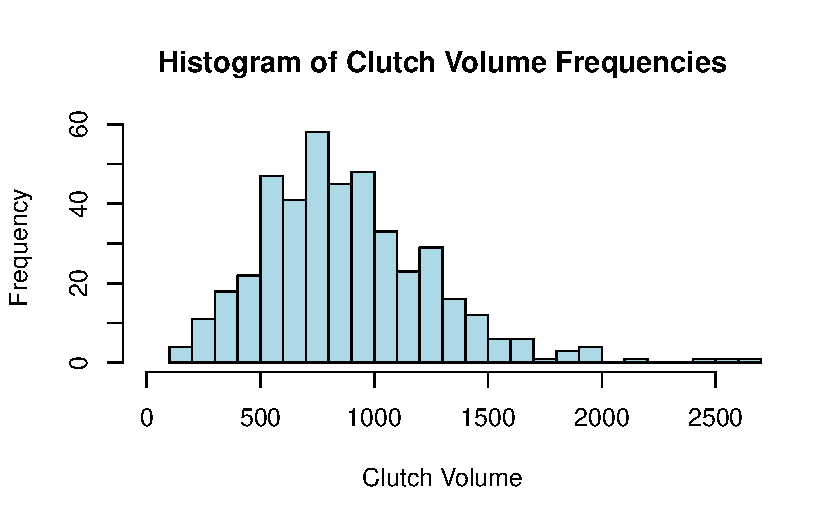
\includegraphics[width=\maxwidth]{figure/unnamed-chunk-16-1} 

\end{knitrout}

\subsubsection{Boxplots}
Another way to visualize data is with a boxplot.  The command for doing this in $R$ is \textit{boxplot()}, and it takes the following arguments:
\begin{itemize}
\item $x$: the variable you want to visualize
\item $axes$: a TRUE/FALSE indicator that determines whether or not numbers are shown on the axes
\item $col$: the color you want the fill inside your boxplot to be; if unspecified, it will be white; must be in quotation marks
\item $xlab$: the label you would like the x-axis to have; must be in quotation marks
\item $ylab$: the label you would like the y-axis to have; must be in quotation marks
\item $xlim$: the range of values you would like the x-axis to have; of the form $c(lower bound, upper bound)$; fairly meaningless for a boxplot
\item $ylim$: the range of values you would like the y-axis to have; of the form $c(lower bound, upper bound)$; be careful not to specify too much here because you can eliminate data of importance to the boxplot
\item $main$: the title you would like the whole plot to have; must be in quotation marks
\end{itemize}
\begin{centering}
\begin{knitrout}
\definecolor{shadecolor}{rgb}{0.969, 0.969, 0.969}\color{fgcolor}\begin{kframe}
\begin{alltt}
\hlcom{## Simplified Figure 1.17}
\hlkwd{boxplot}\hlstd{(}\hlkwc{x} \hlstd{= frog.altitude.data}\hlopt{$}\hlstd{clutch.volume,} \hlkwc{ylab} \hlstd{=} \hlstr{'Clutch Volume'}\hlstd{,} \hlkwc{axes} \hlstd{=} \hlnum{TRUE}\hlstd{,}
        \hlkwc{ylim} \hlstd{=} \hlkwd{range}\hlstd{(frog.altitude.data}\hlopt{$}\hlstd{clutch.volume))}
\end{alltt}
\end{kframe}
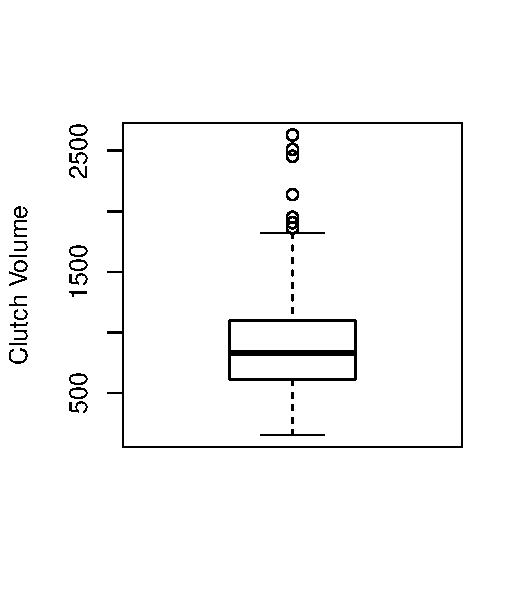
\includegraphics[width=\maxwidth]{figure/unnamed-chunk-17-1} 

\end{knitrout}
\end{centering}

\subsubsection{Scatterplots}
Scatterplots can be used to visualize the relationship between two variables or to visualize just one variable individually.

The command for doing this is \textit{plot()}, and this function takes several arguments:
\begin{itemize}
\item $x$: the first variable you want to visualize; \textit{necessary to include}
\item $y$: the second variable you may want to visualize; included if you want to consider two variables \textit{not necessary to include}
\item $col$: the color you want your dots on the plot to be; if unspecified, they will be black; must be in quotation marks
\item $type$: specifies how you want R to plot the data; if unspecified, you will end up with dots (in a scatterplot); other options include $"l"$ for lines between data points
\item $xlab$: the label you would like the x-axis to have; must be in quotation marks
\item $ylab$: the label you would like the y-axis to have; must be in quotation marks
\item $xlim$: the range of values you would like the x-axis to have; of the form $c(lower bound, upper bound)$
\item $ylim$: the range of values you would like the y-axis to have; of the form $c(lower bound, upper bound)$
\item $main$: the title you would like the whole plot to have; must be in quotation marks
\end{itemize}

The \textit{plot} command has an interesting feature that you can either specify your $x$ and $y$ variables by running $plot(x,y)$ or by running $plot(y~x)$.  Either command will give the same result.  Below provides an example of using the \textit{plot} command for one and two variables (corresponds to Figure 1.18 in the text):
\begin{centering}
\begin{knitrout}
\definecolor{shadecolor}{rgb}{0.969, 0.969, 0.969}\color{fgcolor}\begin{kframe}
\begin{alltt}
\hlcom{# For one variable}
\hlkwd{plot}\hlstd{(frog.altitude.data}\hlopt{$}\hlstd{clutch.volume)}
\end{alltt}
\end{kframe}
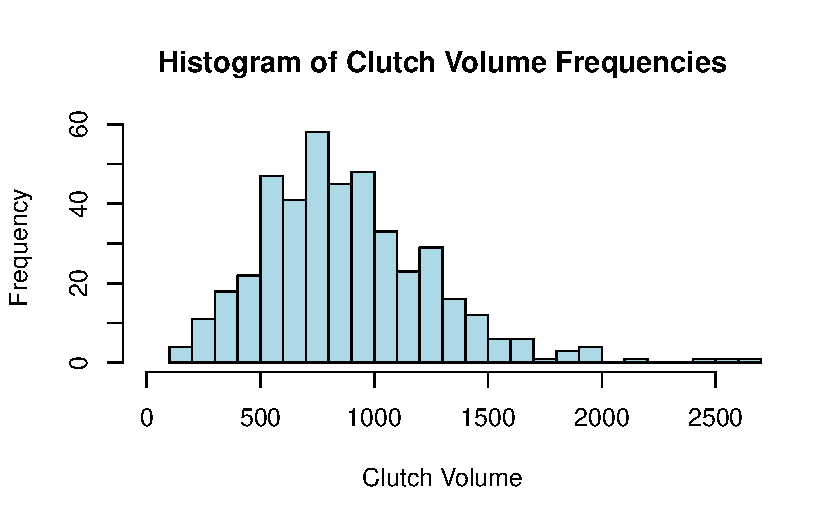
\includegraphics[width=\maxwidth]{figure/unnamed-chunk-18-1} 
\begin{kframe}\begin{alltt}
\hlcom{## Figure 1.18}
\hlcom{# For two variables,}
\hlkwd{plot}\hlstd{(frog.altitude.data}\hlopt{$}\hlstd{clutch.volume}\hlopt{~}\hlstd{frog.altitude.data}\hlopt{$}\hlstd{body.size,}
     \hlkwc{xlab} \hlstd{=} \hlstr{"Female Body Size (cm)"}\hlstd{,} \hlkwc{ylab} \hlstd{=} \hlkwd{expression}\hlstd{(}\hlstr{"Clutch Volume"} \hlopt{~} \hlstd{(mm}\hlopt{^}\hlnum{3}\hlstd{)))}
\end{alltt}
\end{kframe}
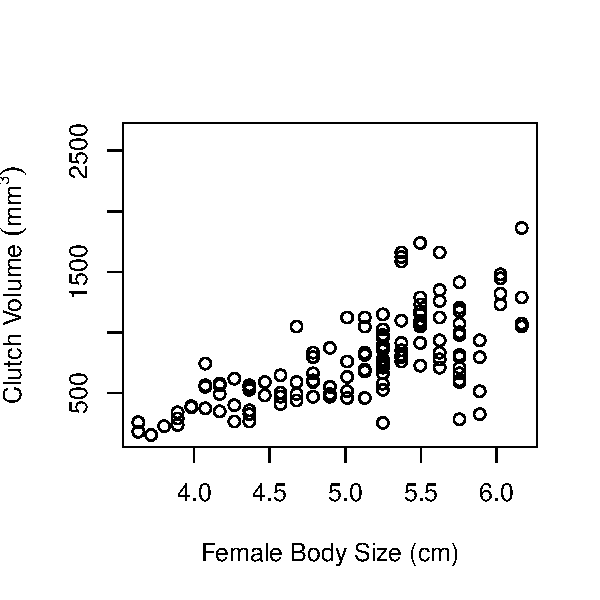
\includegraphics[width=\maxwidth]{figure/unnamed-chunk-18-2} 

\end{knitrout}
\end{centering}

\subsection{Correlation}
Correlation can be calculated by hand but it's a tedious calculation, so doing it using $R$ is often the best bet.  It can be done with the command \textit{cor()} which takes as its arguments your two variables of interest.  Using the example from the text, we can create Figure 1.22 and calculate the correlation as follows:
\begin{knitrout}
\definecolor{shadecolor}{rgb}{0.969, 0.969, 0.969}\color{fgcolor}\begin{kframe}
\begin{alltt}
\hlcom{## Figure 1.22}
\hlstd{x} \hlkwb{=} \hlkwd{c}\hlstd{(}\hlnum{1}\hlstd{,} \hlnum{2}\hlstd{,} \hlnum{3}\hlstd{)}
\hlstd{y} \hlkwb{=} \hlkwd{c}\hlstd{(}\hlnum{5}\hlstd{,} \hlnum{4}\hlstd{,} \hlnum{0}\hlstd{)}

\hlkwd{plot}\hlstd{(x,y)}
\end{alltt}
\end{kframe}
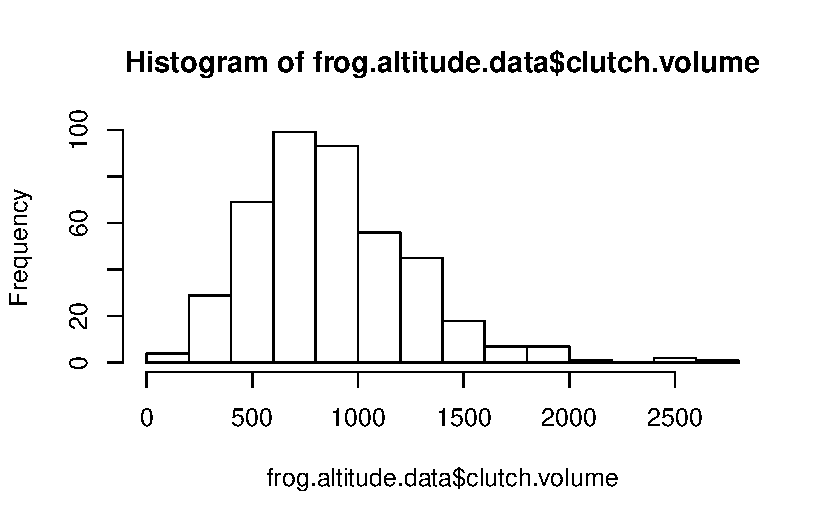
\includegraphics[width=\maxwidth]{figure/unnamed-chunk-19-1} 
\begin{kframe}\begin{alltt}
\hlkwd{cor}\hlstd{(x,y)}
\end{alltt}
\begin{verbatim}
## [1] -0.9449112
\end{verbatim}
\end{kframe}
\end{knitrout}

Figure 1.21 can also be seen with the following with the correlation calculated as stated in the book to be 0.63.  Note that this correlation command contains the argument \textit{use = "complete.obs"}, which simply allows for the correlation calculation by ignoring any NA values in the dataset.
\begin{knitrout}
\definecolor{shadecolor}{rgb}{0.969, 0.969, 0.969}\color{fgcolor}\begin{kframe}
\begin{alltt}
\hlkwd{cor}\hlstd{(life.expectancy.income}\hlopt{$}\hlstd{income, life.expectancy.income}\hlopt{$}\hlstd{life.expectancy,}
    \hlkwc{use} \hlstd{=} \hlstr{"complete.obs"}\hlstd{)}
\end{alltt}
\begin{verbatim}
## [1] 0.6308783
\end{verbatim}
\end{kframe}
\end{knitrout}

\subsection{Transforming Data}
Transformations of data are often of interest, and performing them in $R$ is quite easy.  The plot below shows the before and after of a log transformation on the \textit{life expectancy-income} data.  The \textit{log} command in $R$ perform a natural log, or ln, on the data, despite being written as log.
\begin{knitrout}
\definecolor{shadecolor}{rgb}{0.969, 0.969, 0.969}\color{fgcolor}\begin{kframe}
\begin{alltt}
\hlcom{## Figure 1.24}
\hlkwd{par}\hlstd{(}\hlkwc{mfrow} \hlstd{=} \hlkwd{c}\hlstd{(}\hlnum{1}\hlstd{,} \hlnum{2}\hlstd{))}  \hlcom{## this line just allows two plots to print at the same time}
\hlkwd{hist}\hlstd{(life.expectancy.income}\hlopt{$}\hlstd{income,} \hlkwc{breaks} \hlstd{=} \hlnum{12}\hlstd{,} \hlkwc{xlab} \hlstd{=} \hlstr{"Income (USD)"}\hlstd{,}
    \hlkwc{ylab} \hlstd{=} \hlstr{"Frequency"}\hlstd{,} \hlkwc{ylim} \hlstd{=} \hlkwd{c}\hlstd{(}\hlnum{0}\hlstd{,} \hlnum{120}\hlstd{),} \hlkwc{main} \hlstd{=} \hlstr{"Untransformed"}\hlstd{)}

\hlkwd{hist}\hlstd{(}\hlkwd{log}\hlstd{(life.expectancy.income}\hlopt{$}\hlstd{income),} \hlkwc{breaks} \hlstd{=} \hlnum{12}\hlstd{,} \hlkwc{xlab} \hlstd{=} \hlstr{"Income (log USD)"}\hlstd{,}
    \hlkwc{ylab} \hlstd{=} \hlstr{"Frequency"}\hlstd{,} \hlkwc{ylim} \hlstd{=} \hlkwd{c}\hlstd{(}\hlnum{0}\hlstd{,} \hlnum{30}\hlstd{),} \hlkwc{main} \hlstd{=} \hlstr{"Log Transformed"}\hlstd{)}
\end{alltt}
\end{kframe}
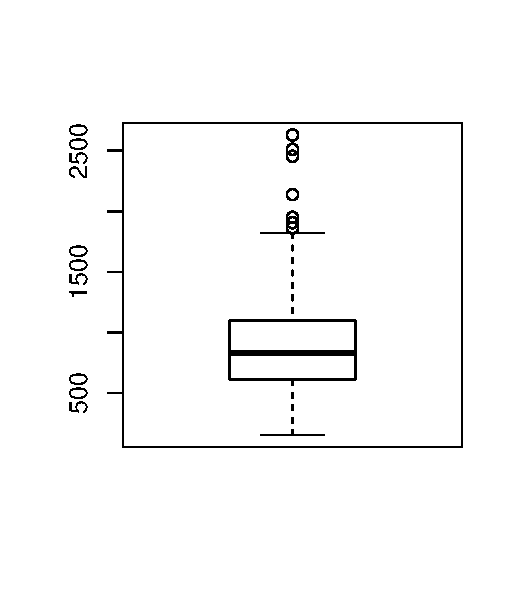
\includegraphics[width=\maxwidth]{figure/unnamed-chunk-21-1} 

\end{knitrout}

Figures 1.21 and 1.25 in the text can be seen below next to each other to see how the log transformation changes a scatterplot.  The function \textit{par()} creates partitions in the graphing output.  In this case, we get 1 row and 2 columns, as indicated by \textit{mfrow = c(1,2)}
\begin{knitrout}
\definecolor{shadecolor}{rgb}{0.969, 0.969, 0.969}\color{fgcolor}\begin{kframe}
\begin{alltt}
\hlcom{## Figure 1.21 and Figure 1.25}
\hlkwd{par}\hlstd{(}\hlkwc{mfrow} \hlstd{=} \hlkwd{c}\hlstd{(}\hlnum{1}\hlstd{,} \hlnum{2}\hlstd{))}
\hlkwd{plot}\hlstd{(life.expectancy.income}\hlopt{$}\hlstd{income,}
    \hlstd{life.expectancy.income}\hlopt{$}\hlstd{life.expectancy,}
    \hlkwc{ylab} \hlstd{=} \hlstr{"Life Expectancy (years)"}\hlstd{,}
    \hlkwc{xlab} \hlstd{=} \hlstr{"Per Capita Income (USD)"}\hlstd{,}
    \hlkwc{main} \hlstd{=} \hlstr{"Untransformed"}\hlstd{)}
\hlkwd{plot}\hlstd{(}\hlkwd{log}\hlstd{(life.expectancy.income}\hlopt{$}\hlstd{income),}
    \hlkwd{log}\hlstd{(life.expectancy.income}\hlopt{$}\hlstd{life.expectancy),}
    \hlkwc{ylab} \hlstd{=} \hlstr{"Life Expectancy (log years)"}\hlstd{,}
    \hlkwc{xlab} \hlstd{=} \hlstr{"Per Capita Income (log USD)"}\hlstd{,}
    \hlkwc{main} \hlstd{=} \hlstr{"Transformed"}\hlstd{)}
\end{alltt}
\end{kframe}
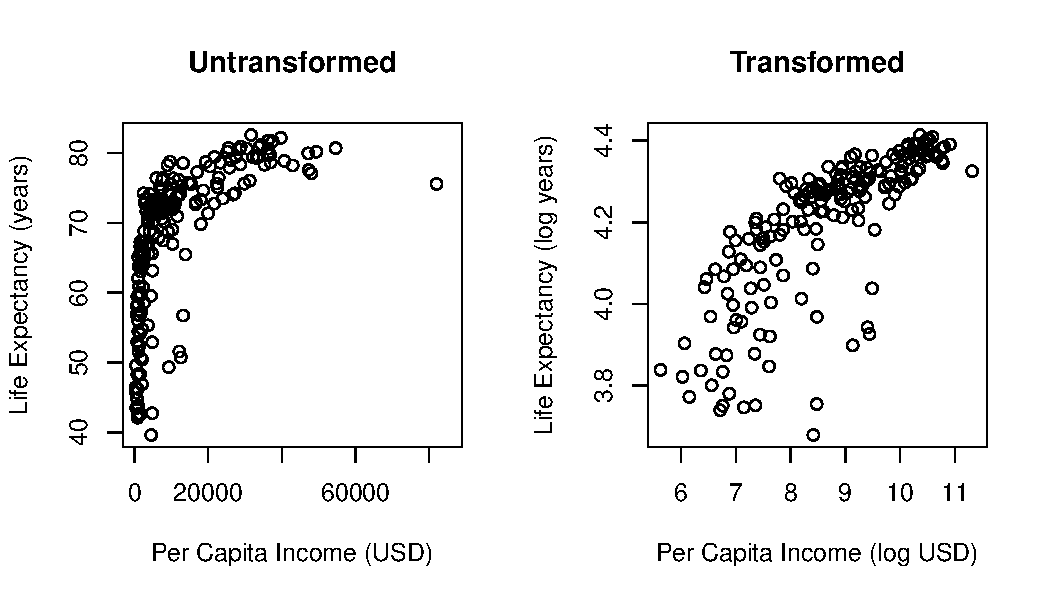
\includegraphics[width=\maxwidth]{figure/unnamed-chunk-22-1} 

\end{knitrout}

\section{Categorical Data}
\subsection{Contingency Tables}
Shown below, Table 1.26 shows a \textbf{frequency table} for genotypes of the actn3.r577x gene.  As a frequency table, it gives the counts of each genotype within the dataset.
\begin{knitrout}
\definecolor{shadecolor}{rgb}{0.969, 0.969, 0.969}\color{fgcolor}\begin{kframe}
\begin{alltt}
\hlcom{## Table 1.26}
\hlkwd{addmargins}\hlstd{(}\hlkwd{table}\hlstd{(famuss}\hlopt{$}\hlstd{actn3.r577x))}
\end{alltt}
\begin{verbatim}
## 
##  CC  CT  TT Sum 
## 173 261 161 595
\end{verbatim}
\end{kframe}
\end{knitrout}
Table 1.27 shows a frequency table on two variables, genotype of the actn3.r577x gene and race from the \textit{famuss} dataset.  Using the command \textit{addmargins} here gives us \textbf{marginal totals}. Because this data summarizes two categorical variables, it is called a \textbf{contingency table}.
\begin{knitrout}
\definecolor{shadecolor}{rgb}{0.969, 0.969, 0.969}\color{fgcolor}\begin{kframe}
\begin{alltt}
\hlcom{## Table 1.27}
\hlkwd{addmargins}\hlstd{(}\hlkwd{table}\hlstd{(famuss}\hlopt{$}\hlstd{race, famuss}\hlopt{$}\hlstd{actn3.r577x))}
\end{alltt}
\begin{verbatim}
##             
##               CC  CT  TT Sum
##   African Am  16   6   5  27
##   Asian       21  18  16  55
##   Caucasian  125 216 126 467
##   Hispanic     4  10   9  23
##   Other        7  11   5  23
##   Sum        173 261 161 595
\end{verbatim}
\end{kframe}
\end{knitrout}

If we instead wanted a contingency table with proportions rather than counts, we could do that in one of two ways - either row proportions or column proportions.  Table 1.28 shows the row proportions and the column proportions are calculated just below.
\begin{knitrout}
\definecolor{shadecolor}{rgb}{0.969, 0.969, 0.969}\color{fgcolor}\begin{kframe}
\begin{alltt}
\hlcom{## Table 1.28}
\hlstd{row.prop.table} \hlkwb{=} \hlkwd{table}\hlstd{(famuss}\hlopt{$}\hlstd{race, famuss}\hlopt{$}\hlstd{actn3.r577x)[}\hlnum{1}\hlopt{:}\hlnum{5}\hlstd{,]}
\hlstd{row.prop.table} \hlopt{/} \hlkwd{rep}\hlstd{(}\hlkwd{rowSums}\hlstd{(row.prop.table),} \hlnum{3}\hlstd{)}
\end{alltt}
\begin{verbatim}
##             
##                     CC        CT        TT
##   African Am 0.5925926 0.2222222 0.1851852
##   Asian      0.3818182 0.3272727 0.2909091
##   Caucasian  0.2676660 0.4625268 0.2698073
##   Hispanic   0.1739130 0.4347826 0.3913043
##   Other      0.3043478 0.4782609 0.2173913
\end{verbatim}
\end{kframe}
\end{knitrout}
Alternatively, we could build a similar table but performing column proportions rather than row proportions as seen in Table 1.29:
\begin{knitrout}
\definecolor{shadecolor}{rgb}{0.969, 0.969, 0.969}\color{fgcolor}\begin{kframe}
\begin{alltt}
\hlcom{## Table 1.29}
\hlstd{col.prop.table} \hlkwb{=} \hlkwd{table}\hlstd{(famuss}\hlopt{$}\hlstd{race, famuss}\hlopt{$}\hlstd{actn3.r577x)[}\hlnum{1}\hlopt{:}\hlnum{5}\hlstd{,]}
\hlstd{col.prop.table} \hlopt{/} \hlkwd{rep}\hlstd{(}\hlkwd{colSums}\hlstd{(col.prop.table),} \hlnum{3}\hlstd{)}
\end{alltt}
\begin{verbatim}
##             
##                      CC         CT         TT
##   African Am 0.09248555 0.03726708 0.01915709
##   Asian      0.08045977 0.10404624 0.09937888
##   Caucasian  0.77639752 0.82758621 0.72832370
##   Hispanic   0.02312139 0.06211180 0.03448276
##   Other      0.02681992 0.06358382 0.03105590
\end{verbatim}
\end{kframe}
\end{knitrout}

\subsection{Bar Plots}
Another way to visualize categorical data is using a \textbf{bar plot}, which can present the data by its categories, and either the count or proportion of occurences within each category.  Note how the \textit{barplot} command takes as its input a table, rather than just a variable.  This is because the data needs to be sorted by its categories before plotting.  We can see Figure 1.30 below which shows two barplots of the same data, sorted on the left by counts and on the right by frequencies.
\begin{knitrout}
\definecolor{shadecolor}{rgb}{0.969, 0.969, 0.969}\color{fgcolor}\begin{kframe}
\begin{alltt}
\hlcom{## Figure 1.30}
\hlkwd{par}\hlstd{(}\hlkwc{mfrow} \hlstd{=} \hlkwd{c}\hlstd{(}\hlnum{1}\hlstd{,} \hlnum{2}\hlstd{))}
\hlkwd{barplot}\hlstd{(}\hlkwd{table}\hlstd{(famuss}\hlopt{$}\hlstd{actn3.r577x))}  \hlcom{## count barplot}
\hlkwd{barplot}\hlstd{(}\hlkwd{table}\hlstd{(famuss}\hlopt{$}\hlstd{actn3.r577x)}\hlopt{/}\hlkwd{sum}\hlstd{(}\hlkwd{table}\hlstd{(famuss}\hlopt{$}\hlstd{actn3.r577x)))}
\end{alltt}
\end{kframe}
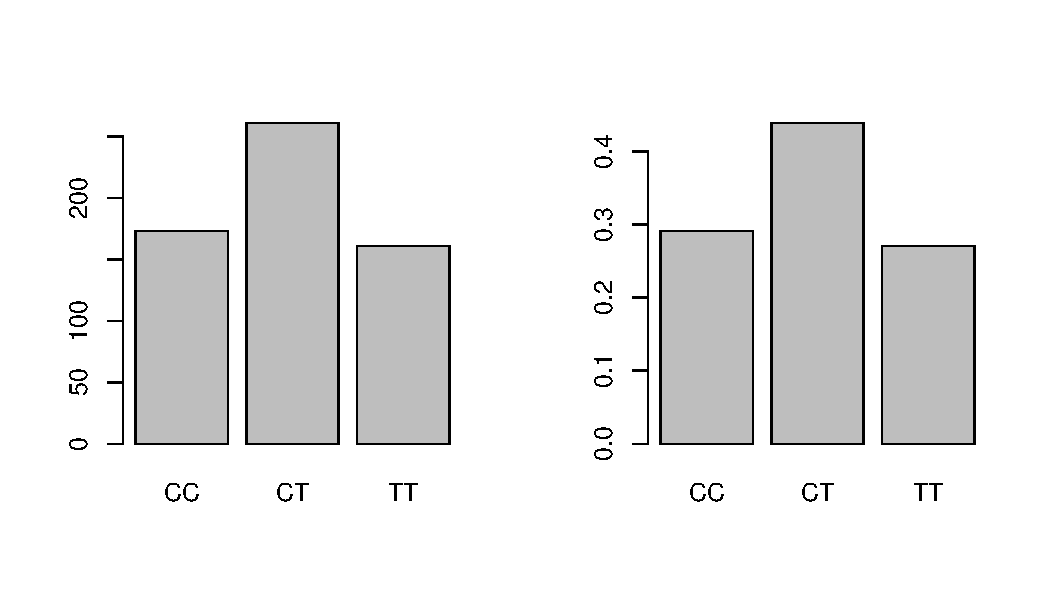
\includegraphics[width=\maxwidth]{figure/unnamed-chunk-27-1} 
\begin{kframe}\begin{alltt}
\hlcom{## frequency barplot}
\end{alltt}
\end{kframe}
\end{knitrout}

\subsubsection{Segmented Bar Plot}
A segmented bar plot is a more sophisticated version of the barplots seen above.  The data is now sorted on two categorical variables, so This code is the most sophisticated thus far, so try to as best as possible work through it line by line.
\begin{knitrout}
\definecolor{shadecolor}{rgb}{0.969, 0.969, 0.969}\color{fgcolor}\begin{kframe}
\begin{alltt}
\hlcom{## Figure 1.31a first, create a table of the data that is}
\hlcom{## sorted}
\hlstd{genotype.race} \hlkwb{=} \hlkwd{matrix}\hlstd{(}\hlkwd{table}\hlstd{(famuss}\hlopt{$}\hlstd{actn3.r577x, famuss}\hlopt{$}\hlstd{race),}
    \hlkwc{ncol} \hlstd{=} \hlnum{3}\hlstd{,} \hlkwc{byrow} \hlstd{= T)}

\hlcom{# second, change the column and row names on the table}
\hlkwd{colnames}\hlstd{(genotype.race)} \hlkwb{=} \hlkwd{c}\hlstd{(}\hlstr{"CC"}\hlstd{,} \hlstr{"CT"}\hlstd{,} \hlstr{"TT"}\hlstd{)}
\hlkwd{rownames}\hlstd{(genotype.race)} \hlkwb{=} \hlkwd{c}\hlstd{(}\hlstr{"African Am"}\hlstd{,} \hlstr{"Asian"}\hlstd{,} \hlstr{"Caucasian"}\hlstd{,}
    \hlstr{"Hispanic"}\hlstd{,} \hlstr{"Other"}\hlstd{)}

\hlcom{# third, plot the barplot where colors are specified}
\hlkwd{barplot}\hlstd{(genotype.race,} \hlkwc{col} \hlstd{=} \hlkwd{c}\hlstd{(}\hlstr{"grey"}\hlstd{,} \hlstr{"red"}\hlstd{,} \hlstr{"blue"}\hlstd{,} \hlstr{"green"}\hlstd{,}
    \hlstr{"yellow"}\hlstd{),} \hlkwc{ylim} \hlstd{=} \hlkwd{c}\hlstd{(}\hlnum{0}\hlstd{,} \hlnum{300}\hlstd{),} \hlkwc{width} \hlstd{=} \hlnum{2}\hlstd{)}
\hlcom{# lastly, include a legend for intepretation of your plots}
\hlkwd{legend}\hlstd{(}\hlstr{"topright"}\hlstd{,} \hlkwc{inset} \hlstd{=} \hlkwd{c}\hlstd{(}\hlnum{0.05}\hlstd{,} \hlnum{0}\hlstd{),} \hlkwc{fill} \hlstd{=} \hlkwd{c}\hlstd{(}\hlstr{"grey"}\hlstd{,} \hlstr{"red"}\hlstd{,}
    \hlstr{"blue"}\hlstd{,} \hlstr{"green"}\hlstd{,} \hlstr{"yellow"}\hlstd{),} \hlkwc{legend} \hlstd{=} \hlkwd{rownames}\hlstd{(genotype.race))}
\end{alltt}
\end{kframe}
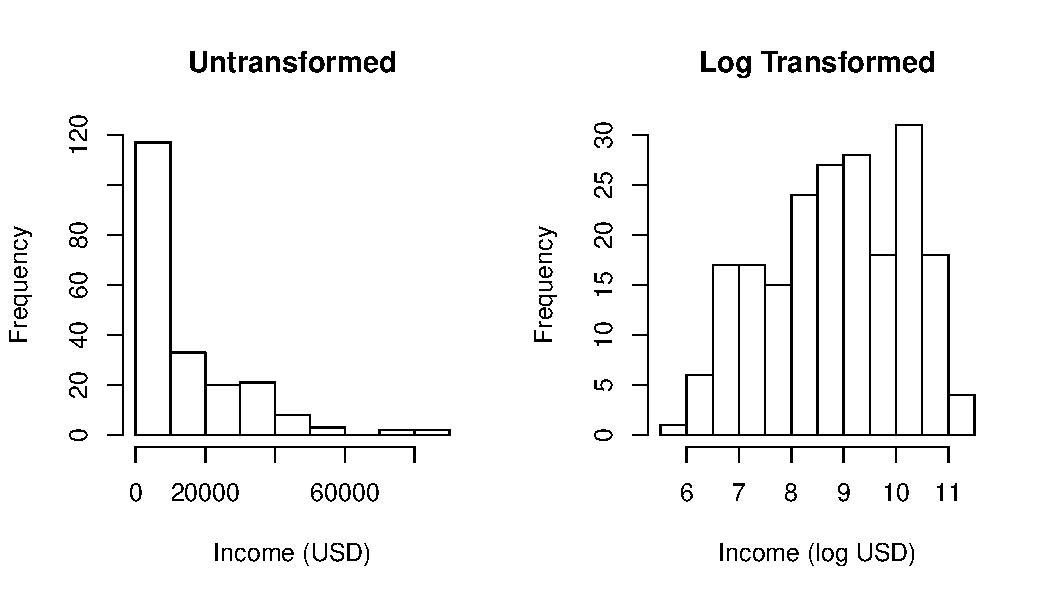
\includegraphics[width=\maxwidth]{figure/unnamed-chunk-28-1} 

\end{knitrout}

If we instead wanted to make a \textbf{standardized segmented bar plot}, we could do that by creating a table of proportions (instead of counts) using the command \textit{prop.table}.  This command is similar to the \textit{table} command but it calculates the proportions for you.  The only difference in the following code from the section above is the use of a proportion table in the first step.
\begin{knitrout}
\definecolor{shadecolor}{rgb}{0.969, 0.969, 0.969}\color{fgcolor}\begin{kframe}
\begin{alltt}
\hlcom{## Figure 1.31b first, create table of proportions}
\hlstd{prop.genotype.race} \hlkwb{<-} \hlkwd{prop.table}\hlstd{(genotype.race,} \hlnum{2}\hlstd{)}

\hlcom{# second, change the column and row names on the table}
\hlkwd{colnames}\hlstd{(prop.genotype.race)} \hlkwb{=} \hlkwd{c}\hlstd{(}\hlstr{"CC"}\hlstd{,} \hlstr{"CT"}\hlstd{,} \hlstr{"TT"}\hlstd{)}
\hlkwd{rownames}\hlstd{(prop.genotype.race)} \hlkwb{=} \hlkwd{c}\hlstd{(}\hlstr{"African Am"}\hlstd{,} \hlstr{"Asian"}\hlstd{,} \hlstr{"Caucasian"}\hlstd{,}
    \hlstr{"Hispanic"}\hlstd{,} \hlstr{"Other"}\hlstd{)}

\hlcom{# second, plot the output}
\hlkwd{barplot}\hlstd{(prop.genotype.race,} \hlkwc{col} \hlstd{=} \hlkwd{c}\hlstd{(}\hlstr{"grey"}\hlstd{,} \hlstr{"red"}\hlstd{,} \hlstr{"blue"}\hlstd{,} \hlstr{"green"}\hlstd{,}
    \hlstr{"yellow"}\hlstd{),} \hlkwc{ylim} \hlstd{=} \hlkwd{c}\hlstd{(}\hlnum{0}\hlstd{,} \hlnum{1.5}\hlstd{),} \hlkwc{width} \hlstd{=} \hlnum{2}\hlstd{)}

\hlcom{# lastly, include a legend for intepretation of your plots}
\hlkwd{legend}\hlstd{(}\hlstr{"topright"}\hlstd{,} \hlkwc{inset} \hlstd{=} \hlkwd{c}\hlstd{(}\hlnum{0.05}\hlstd{,} \hlopt{-}\hlnum{0.005}\hlstd{),} \hlkwc{fill} \hlstd{=} \hlkwd{c}\hlstd{(}\hlstr{"grey"}\hlstd{,}
    \hlstr{"red"}\hlstd{,} \hlstr{"blue"}\hlstd{,} \hlstr{"green"}\hlstd{,} \hlstr{"yellow"}\hlstd{),} \hlkwc{legend} \hlstd{=} \hlkwd{rownames}\hlstd{(prop.genotype.race),}
    \hlkwc{bty} \hlstd{=} \hlstr{"n"}\hlstd{)}
\end{alltt}
\end{kframe}
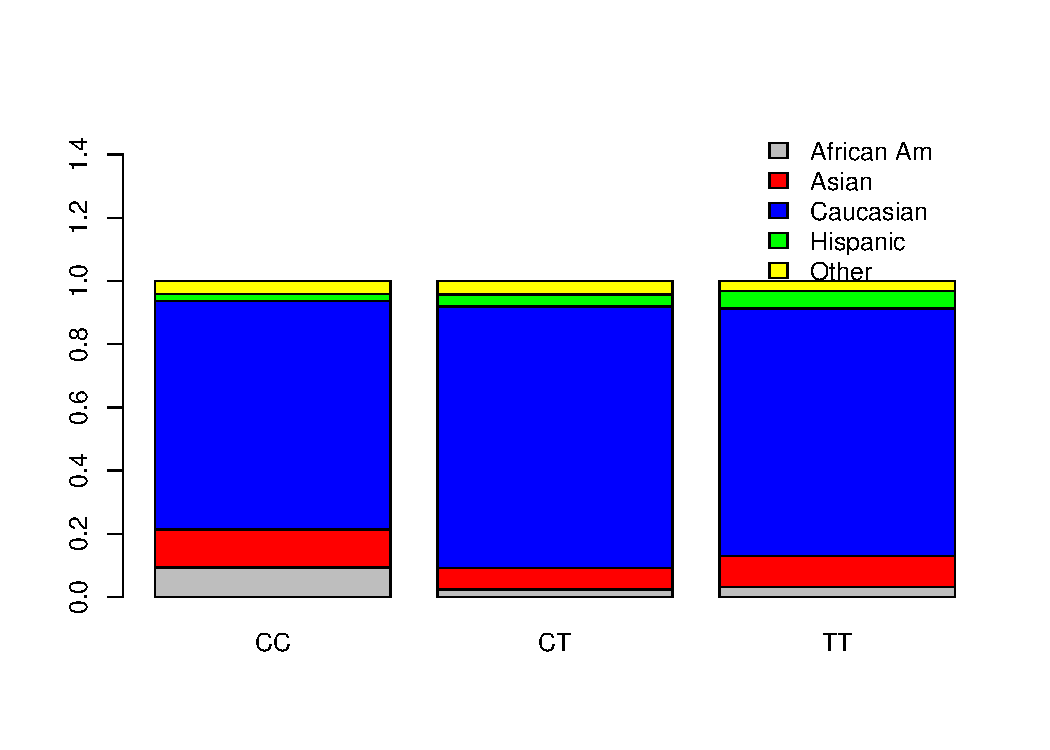
\includegraphics[width=\maxwidth]{figure/unnamed-chunk-29-1} 

\end{knitrout}
\textit{Note:} In the \textit{legend} line, the command  \textit{inset=} controls where on the plot the legend prints out.  Sometimes this specification can be a little bit bizarre so it may require some alteration to find the right spot for the legend.  

If we wanted to reproduce Figure 1.32, where the bars indicate race instead of genotype, we can do the same process as above, with one exception.  In the first step, of creating the table, we must instead put the race variable first as the rows and the gene variable as the columns, as follows:
\begin{knitrout}
\definecolor{shadecolor}{rgb}{0.969, 0.969, 0.969}\color{fgcolor}\begin{kframe}
\begin{alltt}
\hlcom{## Figure 1.32 Plotting two graphs next to each other}
\hlkwd{par}\hlstd{(}\hlkwc{mfrow} \hlstd{= (}\hlkwd{c}\hlstd{(}\hlnum{1}\hlstd{,} \hlnum{2}\hlstd{)))}

\hlcom{# Setting up the table and changing column/row names}
\hlstd{race.genotype} \hlkwb{=} \hlkwd{matrix}\hlstd{(}\hlkwd{table}\hlstd{(famuss}\hlopt{$}\hlstd{race, famuss}\hlopt{$}\hlstd{actn3.r577x),}
    \hlkwc{ncol} \hlstd{=} \hlnum{5}\hlstd{,} \hlkwc{byrow} \hlstd{= T)}
\hlkwd{colnames}\hlstd{(race.genotype)} \hlkwb{=} \hlkwd{c}\hlstd{(}\hlstr{"African Am"}\hlstd{,} \hlstr{"Asian"}\hlstd{,} \hlstr{"Caucasian"}\hlstd{,}
    \hlstr{"Hispanic"}\hlstd{,} \hlstr{"Other"}\hlstd{)}
\hlkwd{rownames}\hlstd{(race.genotype)} \hlkwb{=} \hlkwd{c}\hlstd{(}\hlstr{"CC"}\hlstd{,} \hlstr{"CT"}\hlstd{,} \hlstr{"TT"}\hlstd{)}

\hlcom{# Creating segmented bar plot with a legend}
\hlkwd{barplot}\hlstd{(race.genotype,} \hlkwc{col} \hlstd{=} \hlkwd{c}\hlstd{(}\hlstr{"blue"}\hlstd{,} \hlstr{"green"}\hlstd{,} \hlstr{"yellow"}\hlstd{),} \hlkwc{ylim} \hlstd{=} \hlkwd{c}\hlstd{(}\hlnum{0}\hlstd{,}
    \hlnum{500}\hlstd{),} \hlkwc{width} \hlstd{=} \hlnum{2}\hlstd{)}
\hlkwd{legend}\hlstd{(}\hlstr{"topright"}\hlstd{,} \hlkwc{inset} \hlstd{=} \hlkwd{c}\hlstd{(}\hlnum{0}\hlstd{,} \hlnum{0}\hlstd{),} \hlkwc{fill} \hlstd{=} \hlkwd{c}\hlstd{(}\hlstr{"blue"}\hlstd{,} \hlstr{"green"}\hlstd{,}
    \hlstr{"yellow"}\hlstd{),} \hlkwc{legend} \hlstd{=} \hlkwd{rownames}\hlstd{(race.genotype))}

\hlcom{# Creating standardized segmented bar plot with a legend}
\hlstd{prop.race.genotype} \hlkwb{<-} \hlkwd{prop.table}\hlstd{(race.genotype,} \hlnum{2}\hlstd{)}
\hlkwd{barplot}\hlstd{(prop.race.genotype,} \hlkwc{col} \hlstd{=} \hlkwd{c}\hlstd{(}\hlstr{"blue"}\hlstd{,} \hlstr{"green"}\hlstd{,} \hlstr{"yellow"}\hlstd{),}
    \hlkwc{ylim} \hlstd{=} \hlkwd{c}\hlstd{(}\hlnum{0}\hlstd{,} \hlnum{1.5}\hlstd{),} \hlkwc{width} \hlstd{=} \hlnum{2}\hlstd{)}
\hlkwd{legend}\hlstd{(}\hlstr{"topright"}\hlstd{,} \hlkwc{inset} \hlstd{=} \hlkwd{c}\hlstd{(}\hlnum{0}\hlstd{,} \hlnum{0}\hlstd{),} \hlkwc{fill} \hlstd{=} \hlkwd{c}\hlstd{(}\hlstr{"blue"}\hlstd{,} \hlstr{"green"}\hlstd{,}
    \hlstr{"yellow"}\hlstd{),} \hlkwc{legend} \hlstd{=} \hlkwd{rownames}\hlstd{(race.genotype))}
\end{alltt}
\end{kframe}
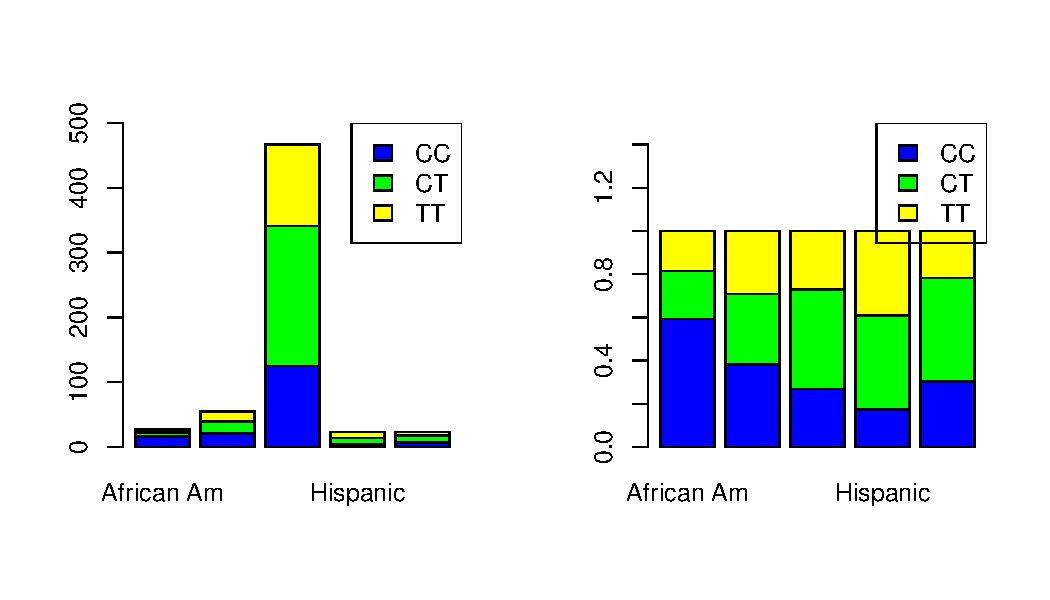
\includegraphics[width=\maxwidth]{figure/unnamed-chunk-30-1} 

\end{knitrout}

\subsubsection{Side-by-Side Boxplots}
With categorical data, you can also create a \textbf{side-by-side boxplot}, as seen in Figure 1.33, which plots the boxplots for corresponding categories on the same plot.  It can be plotted as follows,
\begin{knitrout}
\definecolor{shadecolor}{rgb}{0.969, 0.969, 0.969}\color{fgcolor}\begin{kframe}
\begin{alltt}
\hlcom{## Figure 1.33(a)}
\hlkwd{boxplot}\hlstd{(famuss}\hlopt{$}\hlstd{ndrm.ch} \hlopt{~} \hlstd{famuss}\hlopt{$}\hlstd{actn3.r577x,}
    \hlkwc{ylab} \hlstd{=} \hlstr{"% Change in Non-Dominant Arm Strength"}\hlstd{,}
    \hlkwc{xlab} \hlstd{=} \hlstr{"Genotype"}\hlstd{)}
\end{alltt}
\end{kframe}
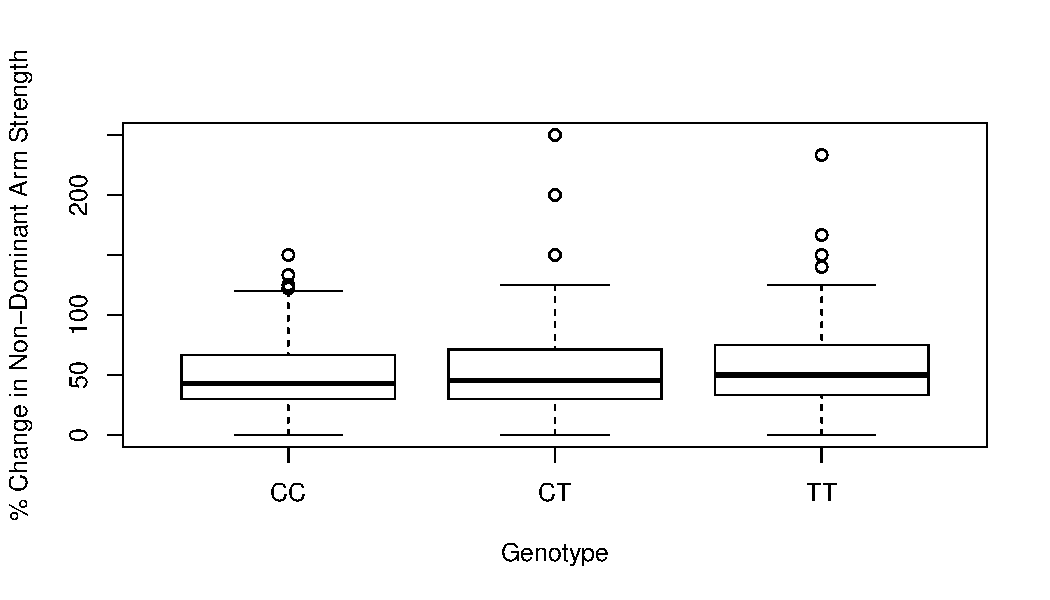
\includegraphics[width=\maxwidth]{figure/unnamed-chunk-31-1} 

\end{knitrout}

Another example of a larger side-by-side boxplot can be seen in Figure 1.34, created as follows,
\begin{knitrout}
\definecolor{shadecolor}{rgb}{0.969, 0.969, 0.969}\color{fgcolor}\begin{kframe}
\begin{alltt}
\hlcom{## Figure 1.34}
\hlkwd{boxplot}\hlstd{(frog.altitude.data}\hlopt{$}\hlstd{clutch.volume} \hlopt{~} \hlstd{frog.altitude.data}\hlopt{$}\hlstd{altitude,}
    \hlkwc{xlab} \hlstd{=} \hlstr{"Clutch Volume"}\hlstd{,} \hlkwc{ylab} \hlstd{=} \hlstr{"Altitude"}\hlstd{)}
\end{alltt}
\end{kframe}
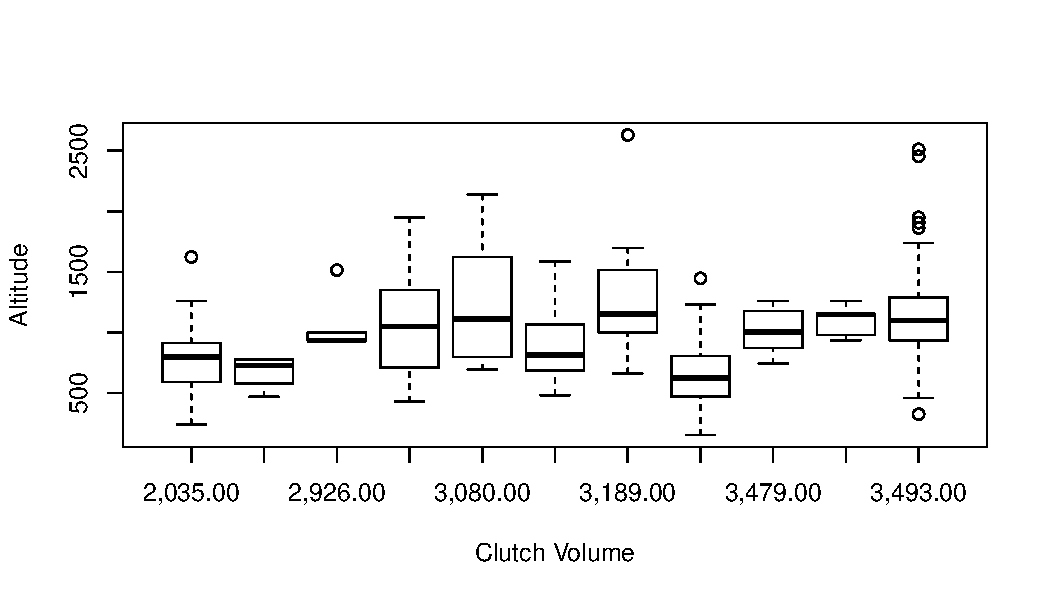
\includegraphics[width=\maxwidth]{figure/unnamed-chunk-32-1} 

\end{knitrout}

\subsubsection{Hollow Histogram}
Using categorical data, we can also plot histograms for each category on top of each other on one single plot, using a \textbf{hollow histogram}.  This can be done as follows,

\begin{knitrout}
\definecolor{shadecolor}{rgb}{0.969, 0.969, 0.969}\color{fgcolor}\begin{kframe}
\begin{alltt}
\hlcom{## Figure 1.33(b)}
\hlkwd{hist}\hlstd{(famuss}\hlopt{$}\hlstd{ndrm.ch[famuss}\hlopt{$}\hlstd{actn3.r577x} \hlopt{==} \hlstr{"CC"}\hlstd{],} \hlkwc{breaks} \hlstd{=} \hlnum{20}\hlstd{,} \hlkwc{border} \hlstd{=} \hlstr{"blue"}\hlstd{,}
    \hlkwc{xlab} \hlstd{=} \hlstr{"% Change in Non-Dominant Arm Strength"}\hlstd{,} \hlkwc{ylim} \hlstd{=} \hlkwd{c}\hlstd{(}\hlnum{0}\hlstd{,} \hlnum{50}\hlstd{),} \hlkwc{xlim} \hlstd{=} \hlkwd{c}\hlstd{(}\hlnum{0}\hlstd{,}
        \hlnum{250}\hlstd{))}
\hlkwd{hist}\hlstd{(famuss}\hlopt{$}\hlstd{ndrm.ch[famuss}\hlopt{$}\hlstd{actn3.r577x} \hlopt{==} \hlstr{"CT"}\hlstd{],} \hlkwc{breaks} \hlstd{=} \hlnum{20}\hlstd{,} \hlkwc{border} \hlstd{=} \hlstr{"green"}\hlstd{,}
    \hlkwc{add} \hlstd{= T)}
\hlkwd{hist}\hlstd{(famuss}\hlopt{$}\hlstd{ndrm.ch[famuss}\hlopt{$}\hlstd{actn3.r577x} \hlopt{==} \hlstr{"TT"}\hlstd{],} \hlkwc{breaks} \hlstd{=} \hlnum{20}\hlstd{,} \hlkwc{border} \hlstd{=} \hlstr{"red"}\hlstd{,}
    \hlkwc{add} \hlstd{= T)}
\end{alltt}
\end{kframe}
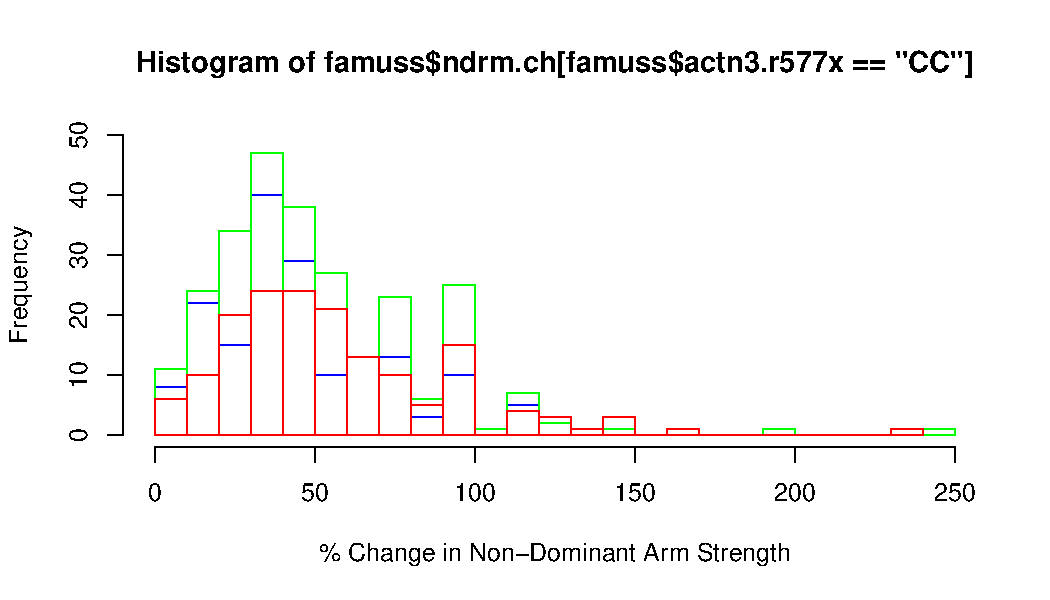
\includegraphics[width=\maxwidth]{figure/unnamed-chunk-33-1} 

\end{knitrout}

\section{Genomic Data}
\begin{knitrout}
\definecolor{shadecolor}{rgb}{0.969, 0.969, 0.969}\color{fgcolor}\begin{kframe}
\begin{alltt}
\hlcom{## Table 1.36}
\hlstd{subset.golub} \hlkwb{=} \hlstd{Golub[}\hlkwd{c}\hlstd{(}\hlnum{1}\hlstd{,} \hlnum{2}\hlstd{,} \hlnum{3}\hlstd{,}
    \hlnum{4}\hlstd{,} \hlnum{5}\hlstd{,} \hlnum{6}\hlstd{),} \hlkwd{c}\hlstd{(}\hlstr{"Samples"}\hlstd{,} \hlstr{"Gender"}\hlstd{,}
    \hlstr{"cancer"}\hlstd{,} \hlstr{"AFFX.BioB.5.at"}\hlstd{,}
    \hlstr{"AFFX.BioB.M.at"}\hlstd{,} \hlstr{"AFFX.BioB.3.at"}\hlstd{)]}
\hlstd{subset.golub}
\end{alltt}
\begin{verbatim}
##    Samples Gender cancer AFFX.BioB.5.at AFFX.BioB.M.at AFFX.BioB.3.at
## 39      39      F   allB     -1363.2764      -1058.585    -541.469194
## 40      40      F   allB      -796.2851      -1167.103       7.538493
## 42      42      F   allB      -679.1392      -1069.832    -690.301829
## 47      47      M   allB     -1164.4002      -1109.940    -990.127218
## 48      48      F   allB     -1299.6538      -1401.999   -1077.543813
## 49      49      M   allB     -1251.6207      -1236.344   -1587.702224
\end{verbatim}
\end{kframe}
\end{knitrout}

\begin{knitrout}
\definecolor{shadecolor}{rgb}{0.969, 0.969, 0.969}\color{fgcolor}\begin{kframe}
\begin{alltt}
\hlcom{## Figure 1.37}
\hlkwd{boxplot}\hlstd{(Golub[,} \hlnum{7}\hlopt{:}\hlnum{9}\hlstd{])}
\end{alltt}
\end{kframe}
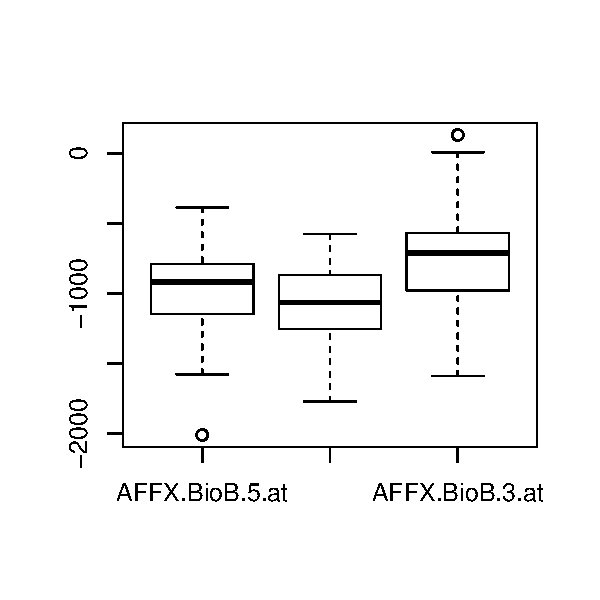
\includegraphics[width=\maxwidth]{figure/unnamed-chunk-35-1} 

\end{knitrout}


\end{document}
